% !TeX root = ../tesis.tex


\chapter{Ajuste con SSKKK}

\label{section:apendix2}

En la Sección \ref{section:optical_properties} se reconstruyó la parte real de la función dieléctrica de los eritrocitos y del plasma mediante la aplicación de las relaciones SSKK. En esta sección se ilustra y discute dicha reconstrucción. En la Fig. \ref{fig:epsLorentz1} se compara la parte real de la función dieléctrica obtenida a partir de SSKK (línea azul continua) con los datos experimentales correspondientes a concentraciones de hemoglobina de 15.3 g/dL y 28.7 g/dL (puntos rojos), observándose desviaciones promedio de 0.024 y 0.03, respectivamente. La línea continua que conecta los puntos experimentales se incluye únicamente como guía para el ojo.
%
\begin{figure}[h]
	\centering
	
	\includegraphics[width=0.45\textwidth]{../../Figuras/ajusteLorentzLegend.pdf}\\
	\sidesubfloat[First image]{\hspace{-0.8cm}{
			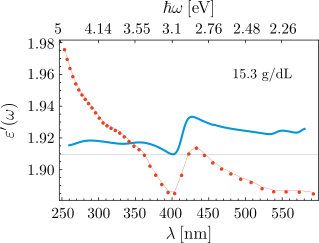
\includegraphics[width=0.47\textwidth]{../../Figuras/sskk15_0.pdf}\label{subfig:ajusteLorentz15}}}\hspace{0.1cm}
	\sidesubfloat[Second image]{\hspace{-0.6cm}{		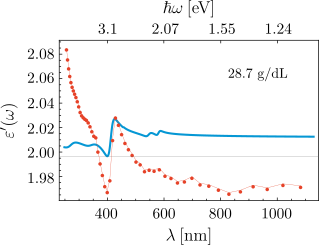
\includegraphics[width=0.47\textwidth]{../../Figuras/sskk28_0.pdf}\label{subfig:ajusteLorentz28}}}	
	\caption{Parte imaginaria de la función dieléctrica como función de la longitud de onda $\lambda$ (eje inferior) y la energía $\hbar\omega$ (eje superior). Se grafican datos experimentales representados por puntos rojos y el ajuste con lorenzianas con una línea azul continua para \textbf{a)} eritrocitos con una concentración de 15.3 g/dL, cuyos experimentales se obtuvieron de \cite{friebelDeterminationComplexRefractive2005a} y \textbf{b)} eritrocitos con una concentración de 28.7 g/dL, cuyos experimentales se obtuvieron de \cite{friebelModelFunctionCalculate2006}. En ambas las figuras las líneas grises verticales indican las frecuencias de resonancia asociadas a los osciladores de Lorentz empleados en el ajuste.}
	\label{fig:epsLorentz1}
\end{figure}
%

De manera análoga, en la Fig. \ref{subfig:epsSSKK_Plasma} se muestra la parte real de la función dieléctrica reconstruida mediante SSKK (línea azul continua) para la concentración de 30.6 g/dL y para el plasma, junto con los datos experimentales (puntos rojos). En estos casos, las desviaciones promedio son del orden de 0.03 para los eritrocitos y de 0.015 para el plasma.

\begin{figure}[]
	\centering
	
	\sidesubfloat[Second image]{\hspace{-0.8cm}{		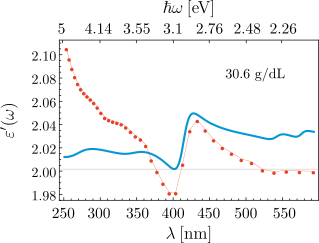
\includegraphics[width=0.47\textwidth]{../../Figuras/sskk30_0.pdf}\label{subfig:ajusteLorentz30}}}\hspace{0.1cm}
	\sidesubfloat[Second image]{\hspace{-0.6cm}{		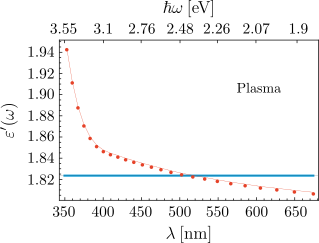
\includegraphics[width=0.47\textwidth]{../../Figuras/sskkPlasma_0.pdf}\label{subfig:ajusteLorentzPlasma}}}
	
	\caption{Parte imaginaria de la función dieléctrica como función de la longitud de onda $\lambda$ (eje inferior) y la energía $\hbar\omega$ (eje superior). Se grafican datos experimentales representados por puntos rojos y el ajuste con lorenzianas con una línea azul continua para \textbf{a)} eritrocitos con una concentración de 30.6 g/dL, cuyos experimentales se obtuvieron de \cite{friebelDeterminationComplexRefractive2005a} y \textbf{b)} plasma, cuyos experimentales se obtuvieron de \cite{meinkeOpticalPropertiesPlatelets2007a}. En ambas las figuras las líneas grises verticales indican las frecuencias de resonancia asociadas a los osciladores de Lorentz empleados en el ajuste.}
	\label{fig:epsLorentz2}
\end{figure}
%